\documentclass{llncs}

\usepackage{llncsdoc}
\usepackage{graphicx,url}
\usepackage[brazil]{babel}
\usepackage[utf8]{inputenc}
\usepackage{float}
\usepackage{setspace}

\usepackage{tabularx}
\usepackage{cite}
\usepackage{hyperref}

\begin{document}
\sloppy
\title{Mezuro: Understading source code metrics}

\author{Rafael Manzo\inst{1}, Diego Camarinha\inst{1},
        Dylan Guedes\inst{1}, Paulo Meirelles\inst{1,2}}

\institute{Instituto de Matemática e Estatística -- Universidade de São Paulo (USP)\\
  Rua do Matão, 1010 -- 05508-090 -- Cidade Universitária -- São Paulo -- SP -- Brasil\\
  \email{\{diegoamc,manzo\}@ime.usp.br}
  \and
  Faculdade do Gama -- Universidade de Brasília (UnB)\\
  Gama -- DF -- Brasil\\
  \email{djmgguedes@gmail.com,paulormm@unb.br}}

\maketitle
\begin{abstract}
  % Contexto
  A facilidade de desenvolvimento e manutenção de um \textit{software} está
diretamente relacionada com a qualidade de seu código-fonte.
  % Problema
  % TODO: adicionar texto que apoie a falta de uso de análise estática em ambientes de desenvolvimento.
  No entanto, analisá-lo impõe dificuldades como, por exemplo, definir as
métricas e interpretar o resultado de uma medição. Além disso, essa prática
ainda não é comum em ambientes de desenvolvimento. Outro problema é a falta de
ferramentas livres que integrem coletores de métricas para diversas liguagens.
  % Soluções propostas
  Neste artigo, apresentamos o Mezuro, uma plataforma \textit{web} livre para a
avaliação colaborativa de código-fonte. O projeto fornece um meio para comparar
projetos e compartilhar conhecimento sobre métricas, ensinando a configurá-las
e interpretá-las. A plataforma foi idealizada de forma que seja possível
integrar diversos coletores de métricas para diversas linguagens. Atualmente, a
ferramenta permite analisar códigos escritos nas linguagens C, C++, Java e
Ruby.
  % Frase de impacto
  Com este projeto, esperamos disseminar o conhecimento e incentivar o uso de
métricas de código.

\textbf{Palavras-chave:} análise estática, métricas de código-fonte,
\textit{software} livre.
\end{abstract}


\section{Introdução} \label{sec:intro}
Métricas de código-fonte estático são medidas extraídas a partir das análises
léxica e sintática deste sem compilá-lo ou executá-lo e podem ser primitivas ou
compostas, ou seja, formadas pela composição de uma ou mais métricas
primitivas. Sua principal função é fornecer informações sobre complexidade,
compreensão, testabilidade, manutenibilidade e evolução do
código REF.

Exemplos de métricas podem ser simples como linhas de código e quantidade de
métodos por classe ou complexas como conexões aferentes de uma classe.  Hoje
existem diversas ferramentas para a simples extração de métricas como
pylint\footnote{\url{http://www.pylint.org/}} (Python),
metric\_fu\footnote{\url{https://github.com/metricfu/metric_fu}} (Ruby) e
Analizo\footnote{\url{http://www.analizo.org/}} (C/C++ e Java), cada uma com
diferentes graus de usabilidade, padrões e conjuntos de métricas, sendo
necessária a criação de uma plataforma que reúna, organize e apresente essas
informações para o usuário.

Por meio da avaliação de métricas de código-fonte podemos definir como está a
qualidade do \textit{software} e pensar em estratégias interessantes para lidar
com a chamada ``crise do \textit{software}'' \cite{naur1969software}. Esta
afirma que, com o crescimento da capacidade computacional, mais problemas
difíceis passam a ter solução viável, mas que, por outro lado, a complexidade
da interface para uso dos novos equipamentos (\textit{hardware}) e do processo
de desenvolvimento atuais combinados com a complexidade dos problemas exacerbam
falhas do \textit{software}. Assim, o controle da qualidade de um
\textit{software} durante sua evolução no tempo torna-se uma ferramenta para
identificar e prevenir tais falhas.

Porém, incorporar esta avaliação às metodologias de desenvolvimento de
\textit{software} não pode ser um processo manual em razão do risco desta
prática cair em desuso. Isto se deve ao fato de que as ferramentas de extração
de métricas, em geral, não apresentam uma interface amigável para seres humanos
lerem seus resultados e muito menos um padrão entre si.  Neste contexto, uma
ferramenta com as seguintes características se faz necessária para a introdução
deste tipo de avaliação constante às metodologias:
\begin{itemize}
  \item interface que agrupe as diversas ferramentas disponíveis;
  \item permita seleção e composição de métricas de forma flexível;
  \item manutenção de um histórico de evolução;
  \item exiba os resultados de forma amigável.
\end{itemize}

%Re-escrever
Por último, como explicado por Meirelles \cite{meirelles2013monitoramento},
ainda não existe um consenso sobre qual conjunto de métricas é relevante para
se avaliar a qualidade do código e muito menos quais valores destas supostas
métricas são bons ou ruins. Portanto, mais uma característica interessante para
uma ferramenta neste campo é que permita aos usuários especialistas definirem
tais parâmetros, viabilizando estudos estatísticos que nos aproximem de uma
conclusão.

\section{Ferramentas similares}
Existem duas ferramentas relacionadas com Mezuro. A primeira, o
SonarQube\footnote{\url{http://www.sonarqube.org/}} é um \textit{software}
livre, licenciado como LGPLv3, que oferece uma plataforma de gerenciamento de
qualidade de código. Por meio de \textit{plugins} disponíveis através de uma
biblioteca\footnote{\url{http://docs.codehaus.org/display/SONAR/Plugin+Library/}}.
Em sua versão básica ele classifica problemas encontrados no código e calcula
métricas simples de cobertura de testes e divida técnica em várias linguagens.
Entretanto, seus melhores \textit{plugins} tem código fechado e pago como, por
exemplo, o para análise de
C/C++\footnote{\url{http://www.sonarsource.com/products/plugins/languages/cpp/}}.

A segunda, o Code Climate\footnote{\url{https://codeclimate.com/}} é uma
ferramenta que fornece análise de códigos JavaScript ou Ruby (da versão 1.8 em
diante) que estejam disponíveis em um servidor Git. O \textit{software} procura
por ``\textit{code smells}'' no programa do usuário e os classifica como mais
ou menos problemáticos levando em consideração o tamanho dos métodos e
duplicação de blocos. Conforme os encontra, o programa atribui valores ao
código para no final determinar uma nota de \textit{A} a \textit{F} com base no
somatório dos valores encontrados. Note que a análise feita não necessariamente
indica um problema real, uma vez que aquela pode ter sido a implementação
escolhida pelo programador.

Recentemente, o Code Climate iniciou uma análise estatística preliminar de
todos os projetos que já foram analisados por este. Publicada informalmente em
uma simples publicação em sua
página\footnote{\url{http://blog.codeclimate.com/blog/2014/05/21/does-team-size-impact-code-quality/?utm\_source=Code+Climate&utm\_campaign=69c024549d-newsletter-NI-2014-05-22&utm\_medium=email&utm\_term=0\_672a7f5529-69c024549d-317410425}}.

\section{The Mezuro project}
\label{sec:mezuro}

O Mezuro é dividido em duas partes: processamento e cálculo de métricas de
código-fonte; e a interface gráfica para apresentação dos resultados. Hoje, o
módulo de processamento de é o Kalibro e o módulo de visualização o Prezento,
sendo o Mezuro o projeto inteiro, ou seja, o Kalibro integrado com o Prezento.


Em seu início como Kalibro, o \textit{software} dispunha de uma interface
gráfica nativa em Java. Porém, logo tomou o rumo de ser um serviço web e assim
essa interface deixou de ser mantida. Para suprir a necessidade de
visualização, foi concebido o projeto então denominado Mezuro
\cite{meirelles2013monitoramento}. Esse projeto visava ser uma rede social na
qual desenvolvedores pudessem calcular métricas de seus códigos-fonte e
compartilhar tanto os resultados quanto a escolha de métricas utilizada. Os
principais objetivos eram disseminar conhecimento sobre métricas e aproximar a
comunidade de um consenso sobre quais delas são mais relevantes para serem
consideradas, em contextos diferentes.
%referenciar artigo do CBSoft 2012

%Falar que o mezuro foi re-escrito
Percebemos que o Mezuro não precisava de todas as funcionalidades de rede
social disponíveis no Noosfero (comunidades, por exemplo) e que elas apenas
adicionavam mais complexidade ao nosso projeto. Reescrevemos o Mezuro como uma
aplicação independente, ou seja, recriar a interface gráfica para o Kalibro.

 Para isso, uma parte considerável do código do plugin foi extraída e
empacotada em uma gema Ruby, denominada \textit{kalibro\_gem}, a licença
\textit{Affero General Public License} versão 3 (AGPLv3) foi adotada e uma
interface completamente redesenhada foi desenvolvida. Nessa interface, o
usuário é o responsável por definir o conjunto de métricas a ser utilizado para
realizar cálculos, com a possibilidade de armazenar os resultados para
comparações futuras. Seu objetivo é:

  \begin{itemize}
    \item Aproximar-se de um consenso acerca de quais métricas devem ser empregadas na análise da qualidade de um código-fonte;
    \item Buscar os valores dessas métricas que definem a qualidade de um código-fonte.
  \end{itemize}

Com essa nova implementação do Mezuro, que mais tarde seria renomeada com seu
nome atual, Prezento, a estabilidade da interface gráfica finalmente deixou o
nível de protótipo com a expectativa de finalmente ser lançada em produção.
Porém, erros que acreditávamos ser relacionados ao plugin do Noosfero
persistiram na nova versão, levando-nos a conclusão de que a implementação
original do Kalibro em Java possuía falhas.

Realizamos testes de escalabilidade e módulo do sistema que mais exigia
capacidade de processamento era o que calculava e analisava métricas de
repositórios, o Kalibro. Por exemplo, quando usávamos o Prezento, em alguns
casos, os processamentos não terminavam. Em suma, dependendo do número de
requisições recebidas e do número de núcleos que o servidor possuía, o Kalibro
entrava em estado de impasse.

Para resolver isso, a principal dificuldade era a arquitetura monolítica de um sistema grande e complexo como o Kalibro. Por exemplo, uma mudança em um ponto do código culminava na obrigação de mudar outros diversos pontos do código. Assim, no final de 2013, iniciamos reescrita em Ruby, uniformizando todo o Projeto Mezuro na mesma linguagem a partir de então.

%Reescrever
Nesse ponto, já pensávamos em duas vantagens decorrentes da reescrita: maior
modularidade do sistema e, por ser software livre, facilitar o entendimento do
código para novos contribuidores. A reescrita também nos livraria do receio de
encontrar outros problemas de tão difícil resolução quanto o que já tínhamos em
mãos. Por conta de tudo isso, decidimos reescrever o Kalibro e, nos primeiros
meses de 2014, adaptamos todo o projeto para receber a mudança e iniciamos
efetivamente a reescrita do sistema. Com dedicação total da equipe, o processo
de reescrita demorou do final de maio ao final de agosto de 2014 e, melhor que
isso, o problema que tínhamos com o antigo Kalibro foi resolvido. Hoje temos
uma base de processamentos estável com código de fácil manutenibilidade.

\section{Arquitetura}

Desde a sua primeira implementação até a sua reescrita completa, a arquitetura
do sistema evoluiu consideravelmente. Após desacoplarmos o Mezuro do Noosfero,
passamos a ter completa autonomia para usar as tecnologias que julgávamos ser
mais adequadas para os nossos problemas. Preocupamo-nos também em mantê-las
atualizadas para termos as funcionalidades mais novas e a correção de defeitos
antigos. Outra mudança importante foi a adoção do estilo arquitetural de micro
serviços (REF). Com o projeto inteiramente reescrito, evoluímos a arquitetura
para o estado atual (Figura \ref{fig:architecture-2}).

Com o objetivo de ser agradável para o desenvolvedor, buscamos criar um sistema
de simples manutenção que incorpore outras funcionalidades facilmente. Para
isto, visamos:

\begin{itemize}
  \item Minimizar a quantidade de código a ser mantida;
  \item Testar e garantir a qualidade do código;
  \item Modularizar a aplicação em diversos serviços independentes.
\end{itemize}

\begin{figure}[H]
  \centering
    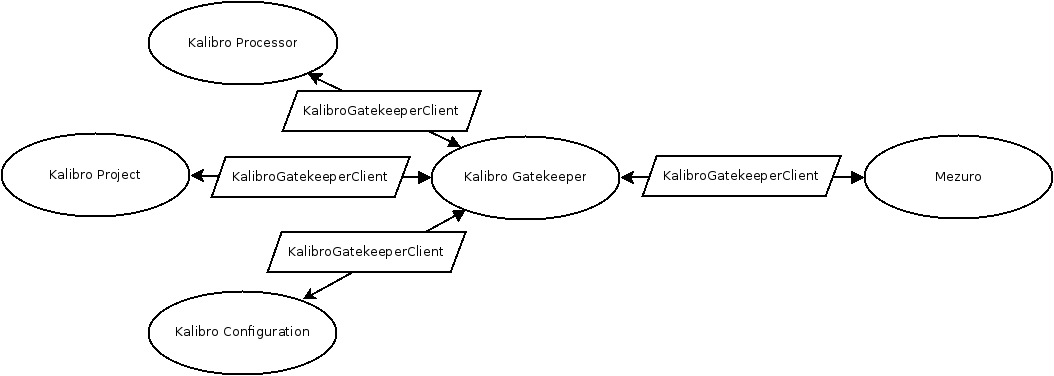
\includegraphics[width=\textwidth]{images/mezuro-architecture-predicted.png}
  \caption{Arquitetura futura do sistema.}
  \label{fig:architecture-2}
\end{figure}

%Possivelmente a figura não é mais do estado atual
A Figura \ref{fig:architecture-2} especifica o atual estado do Mezuro. As
elipses são os diferentes \textit{softwares} envolvidos e os paralelogramos as
interfaces de comunicação entre eles. Na base do Mezuro encontra-se o Kalibro,
segmentado em três entidades menores. O objetivo pretendido com quebra da
estrutura monolítica do Kalibro é que sua manutenção e evolução torne-se mais
fácil, sem que todo o sistema seja comprometido.


\section{Why Mezuro?} \label{subsec:motivacao}

As principais motivações para o surgimento de uma ferramenta como o Mezuro são
os seguintes problemas:

\begin{itemize}
    \item Não há parâmetros de comparação consolidados entre projetos;
    \item Existem estudos, mas poucos dados empíricos;
    \item Ainda é dada pouca importância ao monitoramento de código.
\end{itemize}

Idealizado como uma plataforma de métricas de código, um dos diferenciais do
Mezuro reside na possibilidade de gerar informação sobre o código-fonte de
forma contínua: o usuário decide quando analisar novamente o projeto e
acompanha detalhadamente a evolução das notas ao longo do tempo. Os resultados
de cada análise são públicos, o que permite uma maior transparência entre o
desenvolvedor e a comunidade que utiliza aquele \textit{software}. Assim, ela
pode decidir se aquela solução atende ou não às suas necessidades e se deve
depositar confiança na qualidade do \textit{software} desenvolvido.

No Mezuro, as funcionalidades podem ser divididas em dois grupos:

\begin{itemize}
  \item Projeto
    \begin{itemize}
    \item \textit{Download} do código-fonte a partir de repositórios (Git, Subversion, Bazaar etc) ou via arquivo compactado;
        \item Escolha da periodicidade do processamento do código (1 dia, 2 dias, semanal, quinzenal e mensal);
        \item Escolha de qual configuração de métricas cada repositório irá utilizar;
        \item Nota de cada métrica da configuração para cada arquivo do repositório;
        \item Análise gráfica de cada arquivo do repositório por meio de um gráfico de pontos com notas ao longo do tempo;
        \item Resultados públicos e acessíveis à comunidade.
    \end{itemize}
    \item Configuração
    \begin{itemize}
    \item Criação de configuração e a possibilidade de clonagem;
        \item Estatísticas sobre as configurações mais populares dentro da comunidade;
        \item Criação de intervalos qualitativos associados aos valores das métricas;
        \item Criação de grupos de leitura para a interpretação textual dos resultados das métricas;
        \item Combinações de métricas nativas para criação de análises compostas e mais complexas.
    \end{itemize}
\end{itemize}

O Mezuro tem o formato de uma rede social, no qual os participantes podem ver a
produção de terceiros por meio da avaliação dos projetos ou do clone das
configurações. Essa interação mútua e aberta pode ser interessante para
desenvolvedores, gerentes de projeto, auditores de \textit{software} e até
mesmo uma equipe de desenvolvimento inteira. O objetivo final é criar uma
comunidade que veja o valor de tais metodologias e como isso pode contribuir
para o sucesso do seu projeto.

\section{Conclusão}

O Mezuro surge como uma potencial resposta para a falta de monitoramento e
padronização de código-fonte e a necessidade de avaliação do mesmo,
considerando que é um \textit{software} livre, altamente customizável, com
suporte para muitas linguagens computacionais, interface amigável, que fornece
histórico de processamentos e também com uma arquitetura planejada para
incorporar novas funcionalidades.

\bibliographystyle{splncs03}
\bibliography{mezuro}
\end{document}
